\chapter{Manual de usuario}

\section{Requisitos}

\begin{itemize}
	\item Microsoft Windows 7 o superior
	\item Drivers gráficos compatibles con OpenGL 4
	\item 2GB RAM
\end{itemize}

\section{Instalación}

Instalar usando \texttt{3DCurator.msi} siguiendo los siguientes pasos:

\begin{figure}[H]
	\centering
	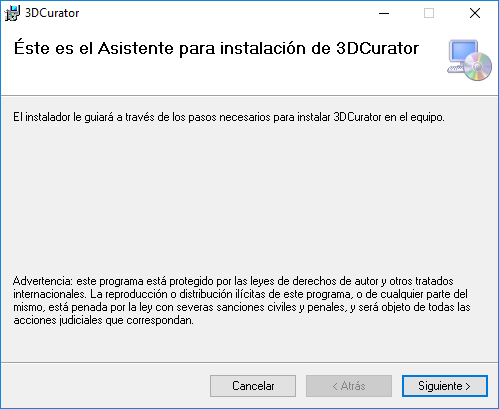
\includegraphics[width=9cm]{imagenes/instalacion_1}
	\caption{Hacer click en Siguiente}
	\label{fig:instalacion_1}
\end{figure}

\begin{figure}[H]
	\centering
	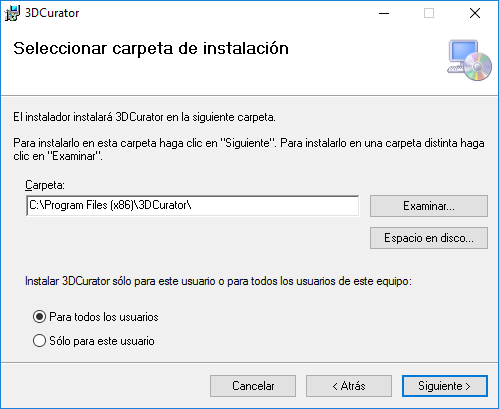
\includegraphics[width=9cm]{imagenes/instalacion_2}
	\caption{Hacer click en Siguiente o cambiar cualquiera de las opciones}
	\label{fig:instalacion_2}
\end{figure}

\begin{figure}[H]
	\centering
	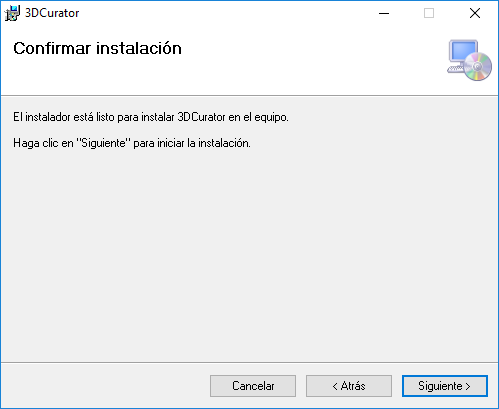
\includegraphics[width=9cm]{imagenes/instalacion_3}
	\caption{Hacer click en Siguiente, dar permisos de administrador y comenzará a instalarse}
	\label{fig:instalacion_3}
\end{figure}

\begin{figure}[H]
	\centering
	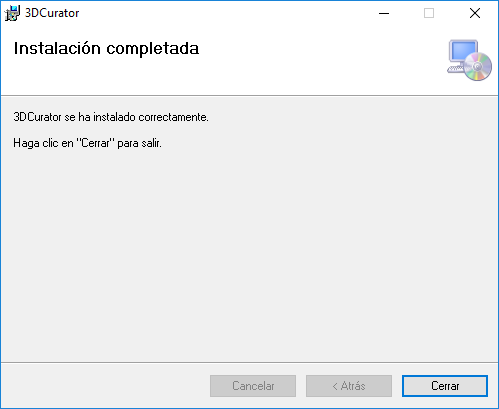
\includegraphics[width=9cm]{imagenes/instalacion_4}
	\caption{Hacer click en Cerrar. Al instalar se habrá creado un acceso directo en el escritorio y en el menú de inicio}
	\label{fig:instalacion_4}
\end{figure}

\section{Capturas de pantalla}

\begin{figure}[H]
	\centering
	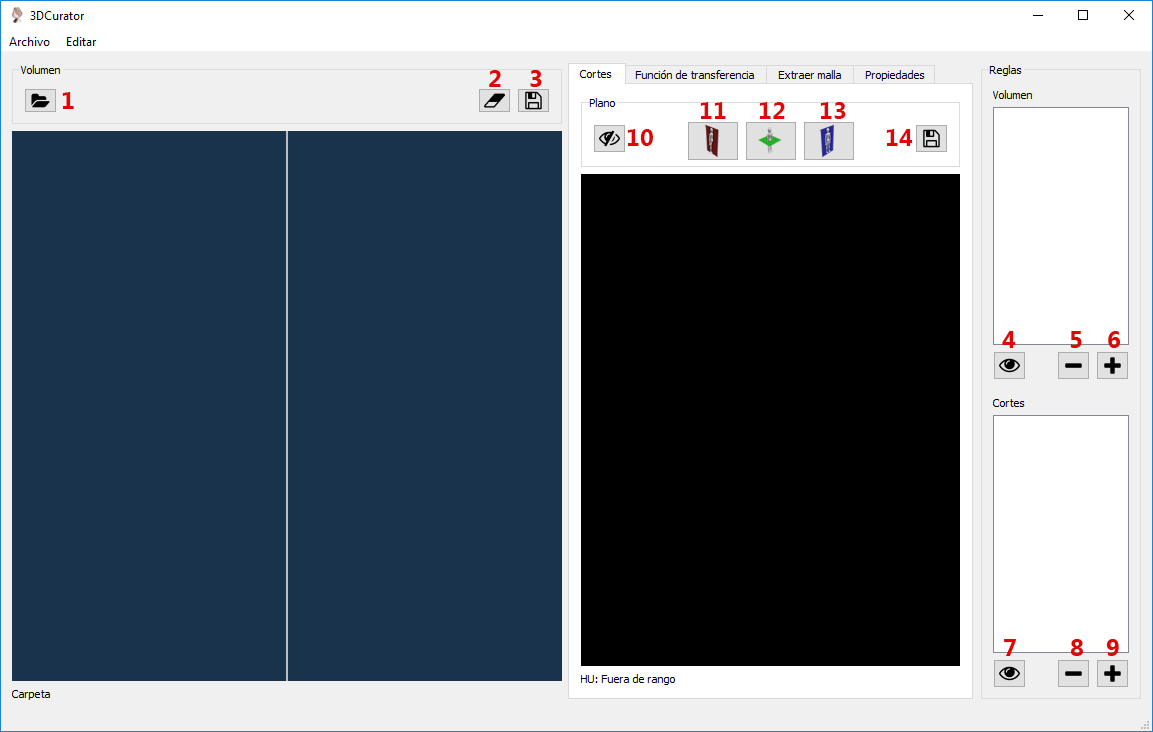
\includegraphics[width=12.5cm]{imagenes/gui_1}
	\caption{Captura de la GUI (Pestaña \textit{Cortes})}
	\label{fig:gui_1}
\end{figure}

\begin{figure}[H]
	\centering
	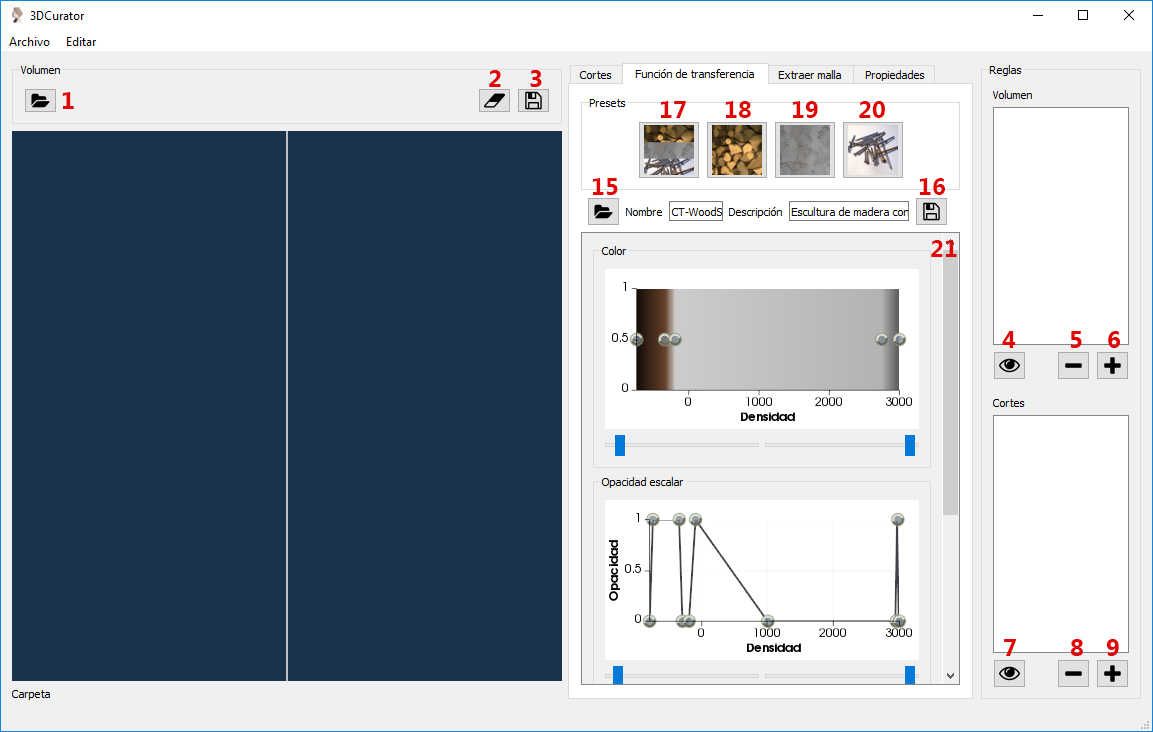
\includegraphics[width=12.5cm]{imagenes/gui_2}
	\caption{Captura de la GUI (Pestaña \textit{Función de transferencia})}
	\label{fig:gui_2}
\end{figure}

\begin{figure}[H]
	\centering
	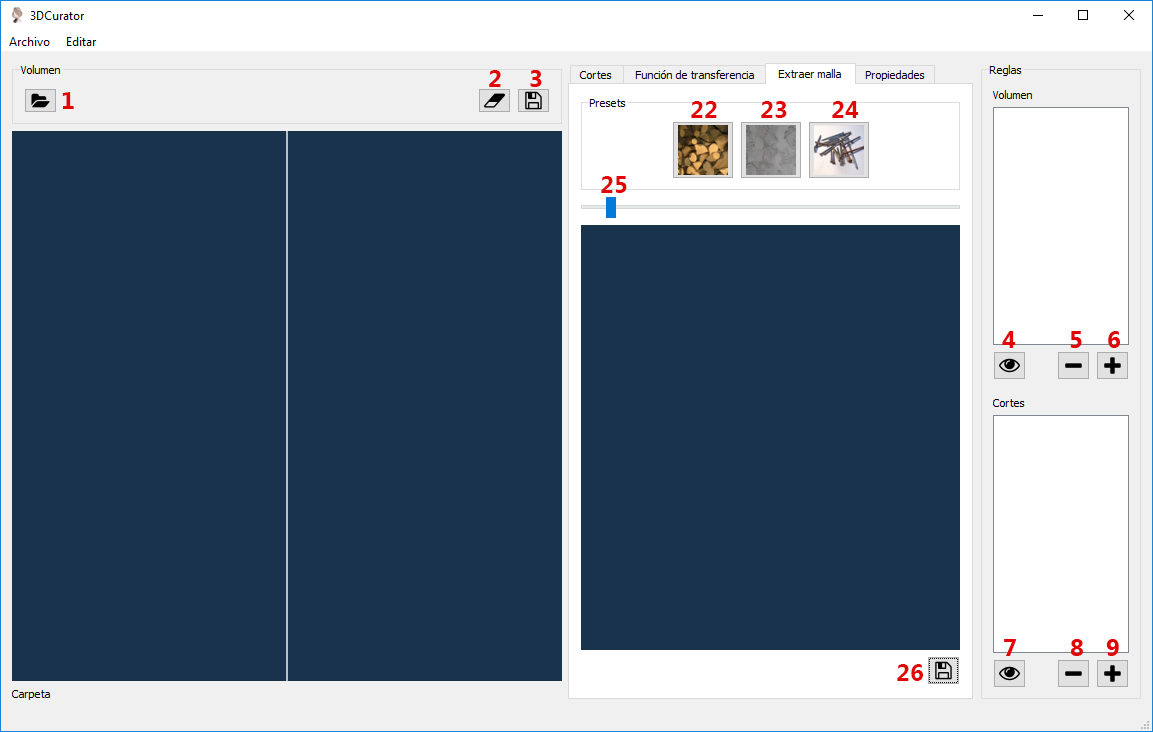
\includegraphics[width=12.5cm]{imagenes/gui_3}
	\caption{Captura de la GUI (Pestaña \textit{Extraer malla})}
	\label{fig:gui_3}
\end{figure}

\begin{figure}[H]
	\centering
	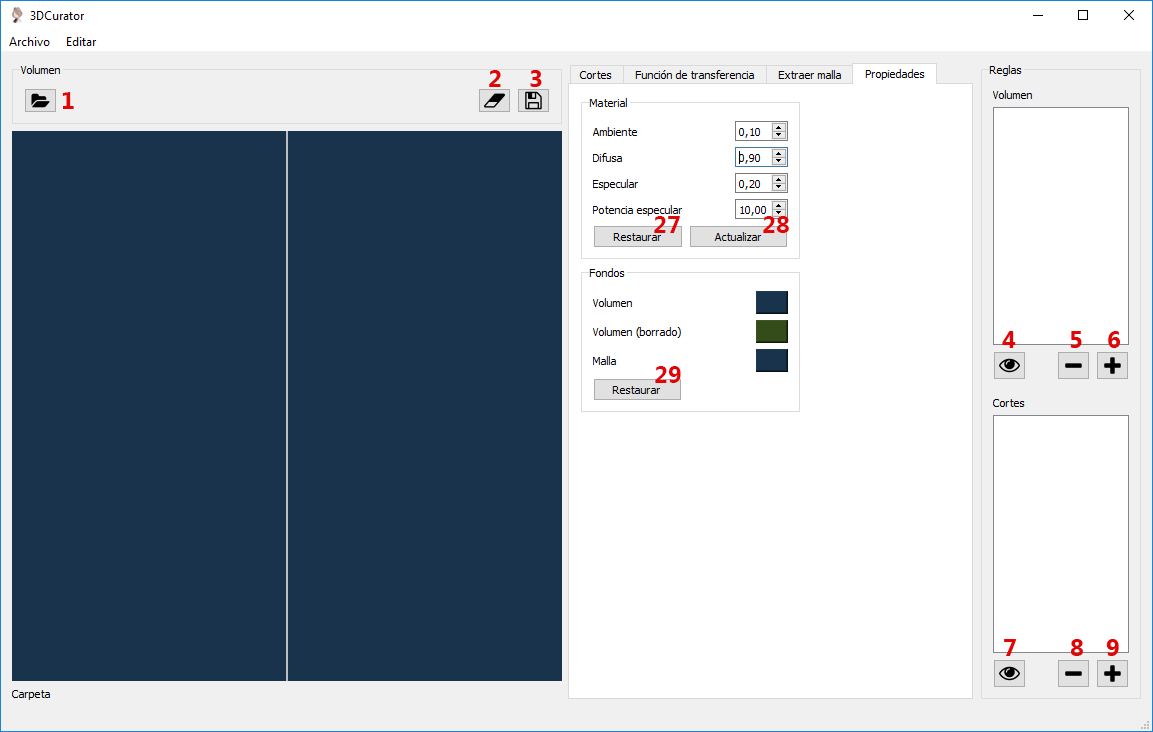
\includegraphics[width=12.5cm]{imagenes/gui_4}
	\caption{Captura de la GUI (Pestaña \textit{Propiedades})}
	\label{fig:gui_4}
\end{figure}

\section{Instrucciones de uso}

\subsection{Abrir directorio DICOM y visualizar datos}

Botón 1, Archivo $ \rangle $ Abrir... o \texttt{Ctrl+O}. Aparecerá una ventana donde se podrá elegir un directorio del sistema. Seleccionar aquel que tenga los archivos DICOM que se quieran importar y pulsar en abrir. Entonces empezará a cargar datos (puede tardar unos segundos). Si hay algún archivo en el directorio que no sea DICOM se mostrará un mensaje de error, pero si ha conseguido cargar el resto se puede continuar con la ejecución del programa sin problema.

Al abrir el archivo DICOM se mostrará la reconstrucción volumétrica en el visor principal, el corte producido con el plano en el visor del plano y la malla en el visor de la malla.

Si se mueve el ratón por el visor del corte, abajo de este aparecerá el valor de densidad del pixel sobre el que está el ratón.

\subsubsection{Visor de volumen y malla}

\begin{itemize}
	\item \textbf{Girar cámara}: Click izdo. + arrastrar
	\item \textbf{Mover cámara}: Click central + arrastrar
	\item \textbf{Zoom}: Click dcho. + arrastrar o rueda del ratón
\end{itemize}

\subsubsection{Visor del corte}

\begin{itemize}
	\item \textbf{Mover}: Click central + arrastrar
	\item \textbf{Zoom}: Click dcho. + arrastrar o rueda del ratón
\end{itemize}

\subsection{Eliminar partes de la figura}

Botón 2, Editar $ \rangle $ Borrar partes o \texttt{Ctrl+May+D}. Se cambiará el visor del volumen de color y no se podrá girar la cámara.

Para borrar hacer click en un punto de la isla que se desea borrar. Entendiendo como isla parte que está separada de las demás. El proceso tardará unos segundos dependiendo del tamaño de la parte que se va a borrar. Al borrar se podrá ver el efecto del borrado y confirmar o volver a como estaba antes de borrar.

En ocasiones se necesitará hacer más de un borrado para borrar una isla por completo.

\subsection{Cambiar plano}

\subsubsection{Mostrar/Esconder}

En la pestaña \textit{Cortes} Botón 10, Editar $ \rangle $ Mostrar/Esconder plano o \texttt{Ctrl+May+H}. Esconderá o mostrará el plano en el visor de volumen. No se actualizará la imagen del corte si se ha escondido hasta que no se vuelva a mostrar.

\subsubsection{Posiciones por defecto}

Para colocarlas centradas en un plano anatómico:

\begin{itemize}
	\item \textbf{Sagital}: En la pestaña \textit{Cortes} Botón 11, Editar $ \rangle $ Plano sagital o \texttt{Ctrl+May+S}
	\item \textbf{Axial}: En la pestaña \textit{Cortes} Botón 12, Editar $ \rangle $ Plano axial o \texttt{Ctrl+May+A}
	\item \textbf{Coronal}: En la pestaña \textit{Cortes} Botón 13, Editar $ \rangle $ Plano coronal o \texttt{Ctrl+May+C}
\end{itemize}

\subsubsection{Mover}

El plano se mueve haciendo click derecho sobre éste y arrastrando hacia donde se desea. Para girarlo hacer el click en los extremos del plano.

\subsection{Guardar imagen del volumen}

Botón 3, Archivo $ \rangle $ Exportar figura... o \texttt{Ctrl+F}. Aparecerá una ventana donde se elegirá dónde, con qué nombre y con qué formato guardar la imagen.

\subsection{Guardar imagen del corte}

En la pestaña \textit{Cortes} Botón 14, Archivo $ \rangle $ Exportar corte... o \texttt{Ctrl+F}. Aparecerá una ventana donde se elegirá dónde, con qué nombre y con qué formato guardar la imagen.
 
\subsection{Cambiar color de fondo de visores}

En la pestaña \textit{Propiedades} pulsar sobre el botón coloreado a la derecha del nombre del visor cuyo color de fondo quiera ser cambiado. Aparecerá una ventana para elegir el color.

Si se desean restaurar los colores por defecto, pulsar en el Botón 29.

\subsection{Cambiar material del volumen}

En la pestaña \textit{Propiedades} cambiar los valores de las distintas componentes del material y pulsar en el Botón 28.

Si se desea restaurar el material por defecto, pulsar en el Botón 27.

\subsection{Función de transferencia}

\subsubsection{Cambiar \textit{preset}}

\begin{itemize}
	\item \textbf{Completo}: En la pestaña \textit{Función de transferencia} Botón 11, Editar $ \rangle $ Preset completo o \texttt{F1}
	\item \textbf{Madera}: En la pestaña \textit{Función de transferencia} Botón 12, Editar $ \rangle $ Preset madera o \texttt{F2}
	\item \textbf{Estuco}: En la pestaña \textit{Función de transferencia} Botón 13, Editar $ \rangle $ Preset estuco o \texttt{F3}
	\item \textbf{Metal}: En la pestaña \textit{Función de transferencia} Botón 14, Editar $ \rangle $ Preset metal o \texttt{F4}
\end{itemize}

\subsubsection{Importar}

En la pestaña \textit{Función de transferencia} Botón 15, Herramientas $ \rangle $ Importar preset... o \texttt{Ctrl+May+I}. Aparecerá una ventana donde se podrá escoger el archivo XML con el \textit{preset} que se quiere importar.

En la pestaña \textit{Propiedades} cambiar los valores de las distintas componentes del material y pulsar en el Botón 28.

Si se desea restaurar el material por defecto, pulsar en el Botón 27.

\subsubsection{Exportar}

Editar nombre y descripción en los campos dedicados para ello y, en la pestaña \textit{Función de transferencia} Botón 16, Herramientas $ \rangle $ Exportar preset... o \texttt{Ctrl+May+E}. Aparecerá una ventana donde se podrá escoger el nombre y la ubicación del archivo con el \textit{preset} que se exportará usando la función de transferencia actual.

\subsubsection{Editar}
 
Interactuar con las tres gráficas de la Caja 21 en la pestaña \textit{Función de transferencia}. Se puede cambiar el rango máximo y mínimo que aparece en la gráfica con los \textit{sliders} inferiores. Para cambiar los puntos: 

\begin{itemize}
	\item \textbf{Añadir punto}: Click
	\item \textbf{Seleccionar punto}: Click sobre el punto
	\item \textbf{Eliminar punto}: Click central sobre el punto o seleccionar y \texttt{Del} o \texttt{Supr}.
	\item \textbf{Mover punto}: Seleccionar punto y arrastrar
	\item \textbf{Cambiar color}: (Solo en la de color) Doble click. Aparecerá una ventana de selección de color
\end{itemize}

\subsection{Generar malla}

En la pestaña \textit{Extraer malla} usar el Slider 25 para cambiar el valor de isosuperficie. Se generará en unos segundos la malla.

Para elegir entre cualquiera de los \textit{presets}:

\begin{itemize}
	\item \textbf{Madera}: En la pestaña \textit{Extraer malla} Botón 22, Editar $ \rangle $ Malla madera. Incluye los materiales madera, estuco y metal.
	\item \textbf{Estuco}: En la pestaña \textit{Extraer malla} Botón 23, Editar $ \rangle $ Malla estuco. Incluye los materiales estuco y metal.
	\item \textbf{Metal}: En la pestaña \textit{Extraer malla} Botón 24, Editar $ \rangle $ Malla metal. Incluye el material metal.
\end{itemize}

\subsection{Extraer malla}

En la pestaña \textit{Extraer malla} Botón 26, Herramientas $ \rangle $ Extraer malla... o \texttt{Ctrl+May+M}. Aparecerá una ventana donde se elegirá el nombre y la ubicación de la malla que se exportará en formato STL.

\subsection{Realizar medidas}

\subsubsection{Añadir regla}

Según el visor donde se realizará la medida pulsar el botón 6 (visor de volumen) o 9 (visor de cortes). Se hará click derecho en el punto inicial y en el final y aparecerá la medida en milímetros.

\subsubsection{Eliminar regla}

Seleccionar una regla de cualquiera de las cajas de reglas y pulsar en el botón 5 (reglas de volumen) u 8 (reglas de cortes). La regla desaparecerá.

\subsubsection{Mostrar/Esconder regla}

Seleccionar una regla de cualquiera de las cajas de reglas y pulsar en el botón 4 (reglas de volumen) u 7 (reglas de cortes). La regla se mostrará o se esconderá según su estado previo.

\subsubsection{Mover regla}

Click izquierdo en cualquiera de los puntos inicial o final de una regla y arrastrar el ratón.